\documentclass[UTF8,11pt]{ctexart}
\usepackage[a4paper,margin=22mm]{geometry}
\usepackage{graphicx,enumitem,amssymb,tabularx}
\usepackage[normalem]{ulem}
\usepackage{xeCJKfntef}
\setlength{\parindent}{0pt}
\setlength{\parskip}{.6em}
\sloppy
\begin{document}
\section*{2021年6月英语四级真题(第2套)}
\subsection*{。2 6 四 二}


\subsection*{、,＇，}


\subsection*{年1 月大 学英语 级 考试真题 （}


\subsection*{2 Writing}


\subsection*{Part I (30 minutes)}


\textbf{Directions: For this pa,rt, you are allowed 80 minutes to write an essay titled "Is technology making people} \textbf{缸y? ". The statement given below is for your reference. You should write at least竺Q words but no more than} \textbf{些words.} \textbf{Many studies claim that computers distract people, make them lazy thinkers and even lower their work} \textbf{efficiency.}


Part ][ Listening Comprehension (25 minutes)


\subsection*{Section A}


\textbf{Directions: In this section, you will加ar three news reports. At t加end of e ach news report , you will 加ar} \textbf{two or three questions. Both the news report and t加questions will be spoken only once. After you 加ar a} \textbf{question , you m}匹\textbf{t choose t加best answer from加four choices marked A), B), C) and D). T, 加nmark} \textbf{t加corresponding letter on Answer Sheet 1 with a single line through t加centre.}


\textbf{Questions 1 and 2 are based on the news report you have just heard.}


\noindent\begin{tabularx}{\linewidth}{@{}lXXXX@{}}\textbf{1.} & \textbf{A.} \textbf{See the Pope.} & \textbf{B.} \textbf{Go to Newcastle.} & \textbf{C.} \textbf{Travel to Germany.} & \textbf{D.} \textbf{Tour an Italian city.}\\\end{tabularx}\par

\textbf{2.}


\begin{itemize}[leftmargin=2em,itemsep=.2em,topsep=.4em]\item[A.] \textbf{He was talcen to hospital in an ambulance.}
\item[B.] \textbf{His car hit a sign and was badly damaged.}
\item[C.] \textbf{His GPS system went out of order.}
\item[D.] \textbf{He ended up in the wrong place.}
\end{itemize}

\textbf{Questions 3 and 4 are based on the news report you have just heanl.}


\textbf{3.}


\begin{itemize}[leftmargin=2em,itemsep=.2em,topsep=.4em]\item[A.] \textbf{Scotland will reach the national target in carbon emissions reduction ahead of schedule.}
\item[B.] \textbf{Glasgow City Council has made a deal with ScottishPower on carbon emissions.}
\item[C.] \textbf{Glasgow has pledged to take the lead in reducing carbon emissions in the UK.}
\item[D.] \textbf{First M血ster Nicola Sturgeon urged ScottishPower to reduce carbon emissions.}
\end{itemize}

\textbf{4.}


\begin{itemize}[leftmargin=2em,itemsep=.2em,topsep=.4em]\item[A.] \textbf{Glasgow needs to invest in new technologies to reach its goal.}
\item[B.] \textbf{Glasgow is going to explore new sources of renewable energy.}
\item[C.] \textbf{Stricter regulation is needed in transforming Glasgow's economy.}
\item[D.] \textbf{It's necessary to create more low-emission zones as soon as possible.}
\end{itemize}

\textbf{Questions 5 to 7 are based on the news report you have just heanl.}


\textbf{5.}


\begin{itemize}[leftmargin=2em,itemsep=.2em,topsep=.4em]\item[A.] \textbf{It donates money to overpopulated animal shelters.}
\item[B.] \textbf{It permits employees to bring cats into their office.}
\item[C.] \textbf{It gives 5,000 yen to employees who keep pet cats.}
\item[D.] \textbf{It allows workers to do whatever their hearts desire.}
\end{itemize}

\textbf{6.}


\begin{itemize}[leftmargin=2em,itemsep=.2em,topsep=.4em]\item[A.] \textbf{Keep cats off the street.}
\item[B.] \textbf{Rescue homeless cats.}
\item[C.] \textbf{Volunteer to help in ammal shelters.}
\item[D.] \textbf{Contnbute to a fund for cat protection.\textperiodcentered{}}
\end{itemize}

\textbf{7.}


\begin{itemize}[leftmargin=2em,itemsep=.2em,topsep=.4em]\item[A.] \textbf{It has contributed tremendously to the firm's fame.}
\item[B.] \textbf{It has helped a lot to improve animals' well-being.}
\item[C.] \textbf{It has led some other companies to follow suit.}
\item[D.] \textbf{It has resulted in damage to office equipment.}
\end{itemize}

\subsection*{\textbf{Section B}}


\textbf{Directions: In this section, you will hear two long conversations. At the end of each conversation, you will} \textbf{hear four questions. Both the conversation and the questions will be spoken only once. After you hear a} \textbf{question, you must choose the best answer from the four choices marked A), B), C) and D). Then mark} \textbf{the corresponding letter on Answer Sheet 1 with a single line through the centre.}


\textbf{Questions 8 to 11 are based on the conversation you have just heanl.}


\textbf{8.}


\begin{itemize}[leftmargin=2em,itemsep=.2em,topsep=.4em]\item[A.] Find out where Jimmy is.
\item[B.] \textbf{Borrow money from Jimmy.}
\item[C.] Make friends with Jimmy.
\item[D.] \textbf{Ask Jimmy what is to be done.}
\end{itemize}

\textbf{9.}


\begin{itemize}[leftmargin=2em,itemsep=.2em,topsep=.4em]\item[A.] \textbf{He was unsure what kind of fellow Jimmy was.}
\item[B.] \textbf{He was working on a study project with Jimmy.}
\item[C.] \textbf{He wanted to make a sincere apology to Jimmy.}
\item[D.] \textbf{He wanted to invite her to join in a study project.}
\end{itemize}

\textbf{10.}


\begin{itemize}[leftmargin=2em,itemsep=.2em,topsep=.4em]\item[A.] \textbf{He got a ticket for speeding.}
\item[B.] \textbf{He got his car badly damaged.}
\item[C.] \textbf{He was involved m a traffic accident.}
\item[D.] \textbf{He had an operation for his injury.}
\end{itemize}

\textbf{11.}


\begin{itemize}[leftmargin=2em,itemsep=.2em,topsep=.4em]\item[A.] \textbf{He needed to make some donation to charity.}
\item[B.] \textbf{He found the 60 pounds in his pocket missing.}
\item[C.] \textbf{He wanted to buy a gift for his mother's birthday.}
\item[D.] \textbf{He wanted to conceal something from his parents.}
\end{itemize}

\textbf{Questions 12 to 15 are based on the conversation you have just heanl.}


\noindent\begin{tabularx}{\linewidth}{@{}lXXXX@{}}\textbf{12.} & \textbf{A.} \textbf{Shopping delivery.} & \textbf{B.} \textbf{Shopping online.} & \textbf{C.} \textbf{Where he goes shopping.} & \textbf{D.} \textbf{How often he does shopping.}\\\end{tabularx}\par

\textbf{13.}


\begin{itemize}[leftmargin=2em,itemsep=.2em,topsep=.4em]\item[A.] \textbf{Searching in the aisles.}
\item[B.] \textbf{\_ Dealing with the traffic.}
\item[C.] \textbf{Driving too long a distance.}
\item[D.] \textbf{Getting one's car parked.}
\end{itemize}

\textbf{14.}


\begin{itemize}[leftmargin=2em,itemsep=.2em,topsep=.4em]\item[A.] \textbf{The after-sales service.}
\item[B.] \textbf{The replacement policy.}
\item[C.] \textbf{The quality of food products.}
\item[D.] \textbf{The damage to the packaging.}
\end{itemize}

\textbf{15.}


\begin{itemize}[leftmargin=2em,itemsep=.2em,topsep=.4em]\item[A.] \textbf{It saves money.}
\item[B.] \textbf{It offers more choice.}
\item[C.] \textbf{It increases the joy of shopping.}
\item[D.] \textbf{It is less time-consuming.}
\end{itemize}

\subsection*{\textbf{Section }C}


\textbf{Directions: In this section , you will hear three passages . At the end of each passage , you will hear three or} \textbf{four questions. Both the passage and the questions will be spoken only once. After you hear a question , you} \textbf{must choose the best answer from the four choices marked A) , B) , C) and D) . Then mark the} \textbf{corresponding letter on Answer Sheet 1 with a single line through the centre.}


\textbf{Questions 16 to 18 are based on the passage you have just heard.}


\textbf{16.}


\begin{itemize}[leftmargin=2em,itemsep=.2em,topsep=.4em]\item[A.] \textbf{They have little talent for learning math.}
\item[B.] \textbf{They need medical help for math anxiety.}
\item[C.] \textbf{They need extra help to catch up in the math class.}
\item[D.] \textbf{They have strong negative emotions towards math.}
\end{itemize}

\textbf{17.}


\begin{itemize}[leftmargin=2em,itemsep=.2em,topsep=.4em]\item[A.] \textbf{It will gradually pass away without teachers' help.}
\item[B.] \textbf{It affects low performing children only.}
\item[C.] \textbf{It is related to a child's low intelligence.}
\item[D.] \textbf{It exists mostly among children from poor families.}
\end{itemize}

\textbf{18.}


\begin{itemize}[leftmargin=2em,itemsep=.2em,topsep=.4em]\item[A.] \textbf{Most of them have average to strong math ability.}
\item[B.] \textbf{Most of them get timely help from their teachers.}
\item[C.] \textbf{They will regain confidence with counselling.}
\item[D.] \textbf{They are mostly secondary school students.}
\end{itemize}

\textbf{Questions 19 to 21 are based on the passage you have just heard.}


\textbf{19.}


\begin{itemize}[leftmargin=2em,itemsep=.2em,topsep=.4em]\item[A.] \textbf{Social media addiction is a threat to our health.}
\item[B.] \textbf{Too many people are addicted to smartphones.}
\item[C.] \textbf{Addiction to computer games is a disease.}
\item[D.] \textbf{Computer games can be rather addictive.}
\end{itemize}

\textbf{20.}


\begin{itemize}[leftmargin=2em,itemsep=.2em,topsep=.4em]\item[A.] \textbf{They prioritize their favored activity over what they should do.}
\item[B.] \textbf{They do their favored activity whenever and wherever possible.}
\item[C.] \textbf{They are unaware of the damage their behavior is doing to them.}
\item[D.] \textbf{They are unable to get rid of their addiction without professional help.}
\end{itemize}

\textbf{21.}


\begin{itemize}[leftmargin=2em,itemsep=.2em,topsep=.4em]\item[A.] \textbf{It may be less damaging than previously believed.}
\item[B.] \textbf{There will never be agreement on its harm to people.}
\item[C.] \textbf{It may prove to be beneficial to developing creativity.}
\item[D.] \textbf{There is not enough evidence to classify it as a disease.}
\end{itemize}

\textbf{Questions 22 to 25 are based on the pa芍吨r you have just heard.}


\textbf{22.}


\begin{itemize}[leftmargin=2em,itemsep=.2em,topsep=.4em]\item[A.] \textbf{They are relatively uniform in color and design.}
\item[B.] \textbf{They appear more formal than other passports.}
\item[C.] \textbf{They are a shade of red bordering on brown.}
\item[D.] \textbf{They vary in color from country to country.}
\end{itemize}

\textbf{23.}


\begin{itemize}[leftmargin=2em,itemsep=.2em,topsep=.4em]\item[A.] \textbf{They must endure wear and tear.}
\item[B.] \textbf{They must be of the same size.}
\item[C.] \textbf{They must be made from a rare material.}
\item[D.] \textbf{They must follow some common standards.}
\end{itemize}

\textbf{24.}


\begin{itemize}[leftmargin=2em,itemsep=.2em,topsep=.4em]\item[A.] \textbf{They look more traditional.}
\item[B.] \textbf{They look more official.}
\item[C.] \textbf{They are favored by airlines.}
\item[D.] \textbf{They are easily identifiable.}
\end{itemize}

\noindent\begin{tabularx}{\linewidth}{@{}lXXXX@{}}\textbf{25.} & \textbf{A.} \textbf{For beauty.} & \textbf{B.} \textbf{For variety.} & \textbf{C.} \textbf{For visibility.} & \textbf{D.} \textbf{For security.}\\\end{tabularx}\par

\subsection*{Part ][ Reading Comprehension (40 minutes)}


\subsection*{Section A}


\textbf{Directions: In this section, there is a passage with ten blanks. You are required to select one word for each} \textbf{blank from a list of choices given in a word bank following the passage. Read the passage through carefully} \textbf{d by a letter. Please mark the corresponding} \textbf{拉fore making your choices. 应ch choice in the bank is identifie} \textbf{letter for each item on Answer Sheet 2 with a single line through the centre. You may not use any of加} \textbf{words in the bank more than once.}


\textbf{Social isolation poses more health risks than obesity or smoking 15 cigarettes a day, according to} \textbf{research published by Brigham Young University. The} \textbf{26} \textbf{is that loneliness is a huge, if silent, risk} \textbf{factor.}


\textbf{Loneliness affects physical health in two ways. First, it produces stress hormones that can lead to} \textbf{many health problems. Second, people who live alone are less likely to go to the doctor} \textbf{27 , to}


\textbf{exercise or to eat a healthy diet.}


\textbf{Public health experts in many countries are} \textbf{28} \textbf{how to address widespread loneliness in our} \textbf{society. Last year Britain even appointed a minister for loneliness. "Loneliness} \textbf{29} \textbf{almost every one of} \textbf{us at some point," its minister for loneliness Baroness Barran said. "It can lead to very serious health}


\noindent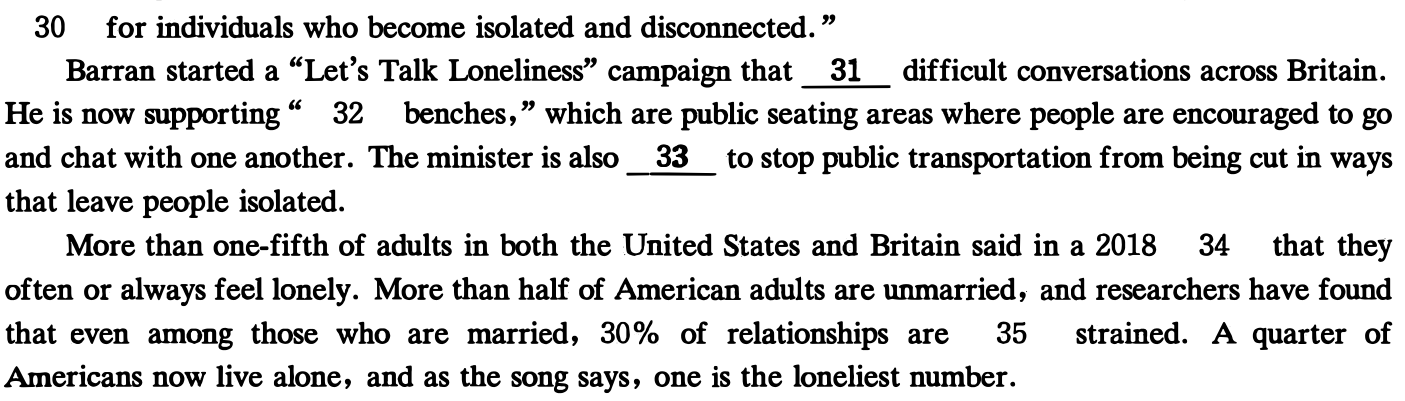
\includegraphics[width=\linewidth,height=.8\textheight,keepaspectratio]{2021-06-02.assets/char-004-line-002.png}\par

\begin{itemize}[leftmargin=2em,itemsep=.2em,topsep=.4em]\item[A.] \textbf{abruptly}
\item[B.] \textbf{appointments}
\item[C.] \textbf{consequences}
\item[D.] \textbf{debating}
\item[E.] \textbf{dimensions}
\item[F.] \textbf{friendly}
\item[G.] \textbf{hindered}
\item[H.] \textbf{idiom}
\item[I.] \textbf{intplication}
\item[J.] \textbf{pushing} \textbf{0) touches}
\item[K.] \textbf{severely}
\item[L.] \textbf{sparked}
\item[M.] \textbf{splitting}
\item[N.] \textbf{survey}
\end{itemize}

\subsection*{Section B}


\textbf{Directions: In this section, you are going to read a passage with ten statements attached to it. Each} \textbf{statement contai}邓\textbf{information given in one of the paragraphs. Identify the paragraph from which the} \textbf{information is derived. You\textperiodcentered{}may choose a paragraph more than once. Each paragraph is marked with a} \textbf{letter. A}心欢\textbf{ir the questions by marking the corresponding letter on Answer Sheet 2.} \textbf{What happens when a language has no words for nmnbers?} \textbf{N Numbers do not exist in all cultures. There are numberless hunter-gatherers in Amazonia, living along}


\textbf{branches of the world's largest river tree. Instead of using words for precise quantities, these people}


\textbf{rely exclusively on terms similar to "a few" or "some." In contrast, our own lives are governed by}


\textbf{numbers. As you read this, you are likely aware of what time it is, how old you are, your checking}


\textbf{account balance, your weight and so on. The exact numbers we think with impact everything in our}


\textbf{lives.}


B) \textbf{But, in a historical sense, number-conscious people like us are the unusual ones. For the bulk of our} \textbf{species' approximately 200,000-year lifespan, we had no means of precisely representing quantities.} \textbf{What's more, the 7,000 or so languages that exist today vary dramatically in how they utilize numbers.}


C) \textbf{Speakers of anumeric, or numberless, languages offer a window into how the invention of numbers} \textbf{reshaped the human experience. Olltures without nwnbers, or with only one or two precise numbers, include} \textbf{the Munduruku and氏啦in Ar}四釭血.\textbf{ Researchers have also studied some adults in Nicaragua who were} \textbf{never taught nmnber words. Without numbers, healthy human adults struggle to precisely distinguish and} \textbf{recall quantities as low as four. In an experiment, a researcher will place nuts into a can one at a time} \textbf{and then remove them one by one. The person watching is asked to signal when all the nuts have been} \textbf{removed. Responses suggest that anumeric people have some trouble keeping track of how many nuts} \textbf{remain in the can, even if there are only four or five in total.}


D) \textbf{This and many other experiments have led to a simple conclusion: When people do not have number} \textbf{words, they struggle to make quantitative distinctions that probably seem natural to someone like you} \textbf{or me. W血e only a small portion of the world's languages are anumeric or nearly anumeric, they} \textbf{demonstrate that number words are not a human universal.}


E) \textbf{It is worth stressing that these anumeric people are cognitively (在认知方面）normal, well-adapted to} \textbf{the surroundings they have dominated for centuries. As a child, I spent some time living with anumeric} \textbf{people, the Piraha who live along the banks of the black Maici River. Like other outsiders, I was} \textbf{continually impressed by their superior understanding of the ecology we shared. Yet numberless people} \textbf{struggle with tasks that require precise discrimination between quantities. Perhaps this should be} \textbf{unsurprising. After all, without counting, how can someone tell whether there are, say, seven or eight} \textbf{coconuts (椰子）in a tree? Such seemingly straightforward distinctions become blurry through numberless} \textbf{eyes.}


F) \textbf{This conclusion is echoed by work with anumeric children in industrialized societies. Prior to being} \textbf{spoon-fed number words, children can only approximately discriminate quantities beyond three. We} \textbf{must be handed the cognitive tools of numbers before we can consistently and easily recognize higher} \textbf{quantities. In fact, acquiring the exact meaning of number words is a painstaking process that takes} \textbf{children years. Initially, kids learn numbers much like they learn letters. They recognize that numbers} \textbf{are organized sequentially, but have little awareness of what each individual number means. With} \textbf{time, they start to understand that a given number represents a quantity greater by one than the} \textbf{number coming before it. This "successor principle" is part of the foundation of our numerical (数字的）cognition, but requires extensive practice to understand.}


G) \textbf{None of us, then, is really a "numbers person." We are not born to handle quantitative distinctions} \textbf{skillfully. In the absence of the cultural traditions that fill our lives with numbers from infancy, we} \textbf{would all struggle with even basic quantitative distinctions. Number words and their written forms} \textbf{transform our quantitative reasoning as they are introduced into our cognitive experience by our} \textbf{parents, peers and school teachers. The process seems so normal that we sometimes think of it as a} \textbf{natural part of growing up, but it is not. Human brains come equipped with certain quantitative} \textbf{instincts that are refined with age, but these instincts are very limited.}


H) \textbf{Compared with other mammals, our numerical instincts are not as remarkable as many assume. We} \textbf{even share some basic instinctual quantitative reasoning with distant non-mammalian relatives like} \textbf{birds. Indeed, work with some other species suggests they too can refine their quantitative thought if} \textbf{they are introduced to the cognitive power tools we call numbers.}


I) \textbf{So, how did we ever invent "unnatural" numbers in the first place? The answer is, literally, at your} \textbf{fingertips. The bulk of the world's languages use base-10, base-20 or base-5 number systems. That is,} \textbf{these smaller numbers are the basis of larger numbers. English is a base-10 or decimal (十进制的）} \textbf{language, as evidenced by words like 14 ("four"+ "10") and 31 ("three" }x \textbf{"10" +"one"). We speak a} \textbf{decimal language because an ancestral tongue, proto-Indo-Buropean, was decimally based. Proto-Inda-} \textbf{European was decimally oriented because, as in so many cultures, our ancestors' hands served as the} \textbf{gateway to the realization that "five fingers on one hand is the same as five fingers on the other. " Such} \textbf{momentary thoughts were represented in words and passed down across generations. This is why the} \textbf{word "five" in many languages is derived from the word for "hand." Most number systems, then, are} \textbf{the by-product of two key factors: the human capacity for language and our inclination for focusing on} \textbf{our hands and fingers. This manual fixation—an indirect by-product of walking upright on two legs—} \textbf{has helped yield numbers in most cultures, but not all.}


J) \textbf{Cultures without numbers also offer insight into the cognitive influence of particular numeric} \textbf{traditions. Consider what time it is. Your day is ruled by minutes and seconds, but these concepts are} \textbf{not real in any physical sense and are nonexistent to numberless people. .Minutes and seconds are the} \textbf{verbal and written representations of an uncommon base-60 number system used in ancient}


\textbf{Mesopotamia. They reside in our minds, numerical artifacts (人工制品）that not all humans inherit}


\textbf{conceptually.}


K) \textbf{Research on the language of numbers shows, more and more, that one of our species' key} \textbf{characteristics is tremendous linguistic (语言的）and cognitive diversity. If we are to truly understand} \textbf{how much our cognitive lives differ cross-culturally, we must continually explore the depths of our} \textbf{species' linguistic diversity.}


\textbf{36. It is difficult for anumeric people to keep track of the change in numbers even when the total is very small.}


\textbf{37. Human numerical instincts are not so superior to those of other mammals as is generally believed.}


\textbf{38. The author emphasizes being anumeric does not affect one's cognitive ability.}


\textbf{39. In the long history of mankind, humans who use numbers are a very small minority.}


\textbf{40. An in-depth study of differences between human languages contributes to a true understanding of}


\textbf{cognitive differences between cultures.}


\textbf{41. A conclusion has been drawn from many experiments that anumeric people have a hard time}


\textbf{distinguishing quantities.}


\textbf{42. Making quantitative distinctions is not an inborn skill.}


\textbf{43. Every aspect of our lives is affected by numbers.}


\textbf{44. Larger numbers are said to be built upon smaller numbers.}


\textbf{45. It takes great efforts for children to grasp the concept of number words.}


\subsection*{\textbf{Section} C}


\textbf{Directions: There are 2 passages in this section. Each passage is followed by some questions or unfinished} \textbf{statements. For each of them there are four choices marked A), B), C) and D). You should decide on the} \textbf{best choice and mark the corresponding letter on Answer Sheet 2 with a single line through the centre.}


\subsection*{\textbf{Passage One}}


\textbf{Questions 46 to SO are based on the following passage.}


\textbf{Sugar shocked. That describes the reaction of many Americans this week following revelations that,} \textbf{50 years ago, the sugar industry paid Harvard scientists for research that shifted the focus away from} \textbf{sugar's role in heart disease-and put the spotlight (注意的中心） squarely on dietary fat.}


\textbf{What might surprise consumers is just how many present-day nutrition studies are still funded by the} \textbf{food industry. Nutrition scholar Marion Nestle of New York University spent a year informally tracking} \textbf{industry-funded studies on food. "Roughly 90\% of nearly 170 studies favored the sponsor's interest,"} \textbf{Nestle tells us. Other systematic reviews support her conclusions.}


\textbf{For instance, studies funded by Welch Foods--the brand behind Welch's 100\% Grape Juice-found} \textbf{that drinking Concord grape juice daily may boost brain function. Another, funded by Qualcer Oats,} \textbf{concluded, as a Daily Mail story put it, that "hot oatmeal (燕麦粥） brealdast keeps you full for longer. "}


\textbf{Last year, The New York Times revealed how Coca七ola was funding well-known scientists and} \textbf{organizations promoting a message that, in the battle against weight gain, people should pay more} \textbf{attention to exercise and less to what they eat and drink. Coca七ola also released data detailing its funding} \textbf{of several medical institutions and associations between 2010 and 2015.}


\textbf{"It's certainly a problem that so much research in nutrition and health is funded by industry," says} \textbf{Bonnie Liebman, director of nutrition at the Center for Science in the Public Interest. "When the food} \textbf{industry pays for research, it often gets what it pays for." And what it pays for is often a pro-industry} \textbf{finding.}


\textbf{Given this environment, consumers should be skeptical (怀疑的） when reading the latest finding in} \textbf{nutrition science and ignore the latest study that pops up on your news feed. "Rely on health experts} \textbf{who've reviewed all the evidence," Liebman says, pointing to the official government Dietary Guidelines,}


\textbf{which are based on reviews of hundreds of studies.}


\textbf{"And that expert advice remains pretty simple," says Nestle. "We know what healthy diets are-一lots} \textbf{of vegetables, not too much junk food, balanced calories. Everything else is really difficult to do} \textbf{experimentally. "}


\noindent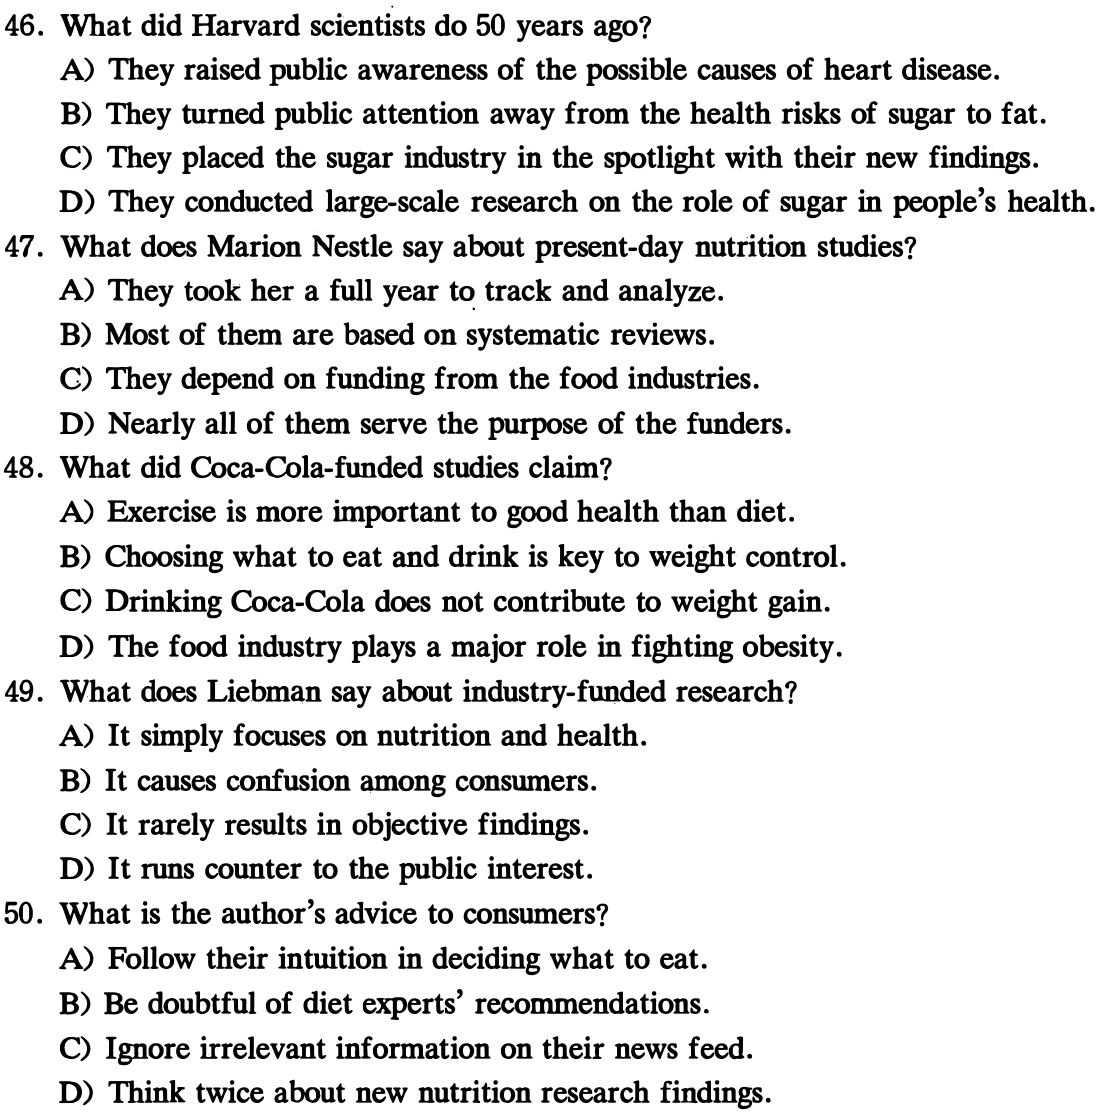
\includegraphics[width=\linewidth,height=.8\textheight,keepaspectratio]{2021-06-02.assets/char-007-line-002.png}\par

46. What did Harvard scientists do 50 years ago?


\begin{itemize}[leftmargin=2em,itemsep=.2em,topsep=.4em]\item[A.] They raised public awareness of the possible causes of heart disease.
\item[B.] They turned public attention away from the health risks of sugar to fat.
\item[C.] They placed the sugar industry in the spotlight with their new findings.
\item[D.] They conducted large-scale research on the role of sugar in people's health.
\end{itemize}

47. What does Marion Nestle say about present-day nutrition studies?


\begin{itemize}[leftmargin=2em,itemsep=.2em,topsep=.4em]\item[A.] They took her a full year to track and analyze.
\item[B.] Most of them are based on systematic reviews.
\item[C.] They depend on funding from the food industries.
\item[D.] Nearly all of them serve the purpose of the funders.
\end{itemize}

48. What did Coca-Cola-funded studies claim?


\begin{itemize}[leftmargin=2em,itemsep=.2em,topsep=.4em]\item[A.] Exercise is more important to good health than diet.
\item[B.] Choosing what to eat and drink is key to weight control.
\item[C.] Drinking Coca-Cola does not contribute to weight gain.
\item[D.] The food industry plays a major role in fighting obesity.
\end{itemize}

49. What does Liebman say about industry-funded research?


\begin{itemize}[leftmargin=2em,itemsep=.2em,topsep=.4em]\item[A.] It simply focuses on nutrition and health.
\item[B.] It causes confusion among consumers.
\item[C.] It rarely results in objective findings.
\item[D.] It runs counter to the public interest.
\end{itemize}

50. What is the author's advice to consumers?


\begin{itemize}[leftmargin=2em,itemsep=.2em,topsep=.4em]\item[A.] Follow their intuition in deciding what to eat.
\item[B.] Be doubtful of diet experts' recommendations.
\item[C.] Ignore irrelevant information on their news feed.
\item[D.] Think twice about new nutrition research findings.
\end{itemize}

\subsection*{\textbf{Passage Two}}


\textbf{Questions 51 to 55 are based on the following passage.}


\textbf{Success was once defined as being able to stay at a company for a long time and move up the corporate} \textbf{ladder. The goal was to reach the top, accumulate wealth and retire to a life of ease. My father is a} \textbf{successful senior executive. In 35 years, he worked for only three companies.}


\textbf{When I started my career, things were already different. If you weren't changing companies every} \textbf{three or four years, you simply weren't getting ahead in your career. But back then, if you were a} \textbf{consultant or freela}砒\textbf{er (自由职业者），people would wonder what was wrong with you. They would} \textbf{assume you had problems getting a job.}


\textbf{Today, consulting or freelancing for five businesses at the same time is a badge of honor. It shows} \textbf{how valuable an individual is. Many companies now look to these "ultimate professionals" to solve} \textbf{problems their full-time teams can't. Or they save money by hiring" top-tier (顶尖的）experts" only for} \textbf{particular projects.}


\textbf{Working at home or in cafes, starting businesses of their own, and even launching business ventures} \textbf{that eventually may fail, all indicate "initiative," "creativity," and "adaptability," which are desirable} \textbf{qualities in today's workplace. Most important, there is a growing recognition that people who balance}


\noindent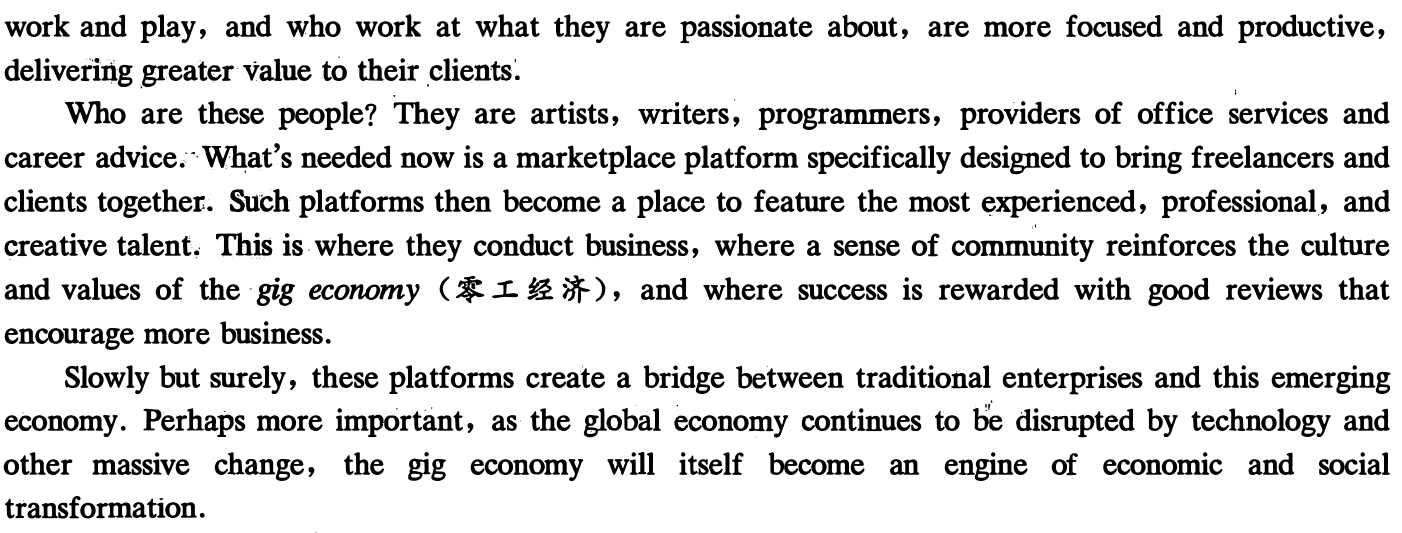
\includegraphics[width=\linewidth,height=.8\textheight,keepaspectratio]{2021-06-02.assets/char-008-line-000.png}\par

\textbf{51. W匝t does the author use the example of his father to illustrate?}


\begin{itemize}[leftmargin=2em,itemsep=.2em,topsep=.4em]\item[A.] \textbf{How long people took to reach the top of their career.}
\item[B.] \textbf{How people accumulated wealth in his father's time.}
\item[C.] \textbf{How people viewed sm:cess in his father's time.}
\item[D.] \textbf{How long people usually stayed in a company.}
\end{itemize}

\textbf{52. Why did people often change jobs when the author started his career?}


\begin{itemize}[leftmargin=2em,itemsep=.2em,topsep=.4em]\item[A.] \textbf{It was considered a fashion at that time.}
\item[B.] \textbf{It was- a way to advance in their career.}
\item[C.] \textbf{It was a response to the changing job market.}
\item[D.] \textbf{It was difficult to keep a job for long.}
\end{itemize}

\textbf{53. What does the author say about people now working for跁veral businesses at the same time?}


\begin{itemize}[leftmargin=2em,itemsep=.2em,topsep=.4em]\item[A.] \textbf{They are often regarded as most treasured talents.}
\item[B.] \textbf{They are. able to bring their potential into fuller play.}
\item[C.] \textbf{They have control over their life and work schedules.}
\item[D.] \textbf{They feel proud of being outstanding problem solver.}
\end{itemize}

\textbf{54. What have businesses come to recognize now?}


\begin{itemize}[leftmargin=2em,itemsep=.2em,topsep=.4em]\item[A.] \textbf{Who is capable of solving problems with ease.}
\item[B.] \textbf{How people can be more focused and productive.}
\item[C.] \textbf{What kind of people can contribute tnore to them.}
\item[D.] \textbf{Why some people are more passionate about work.}
\end{itemize}

\textbf{55. What does the author say about the'gig economy?}


\begin{itemize}[leftmargin=2em,itemsep=.2em,topsep=.4em]\item[A.] \textbf{It may force companies to reform their business practice.}
\item[B.] \textbf{It may soon replace the traditional economic model.}
\item[C.] \textbf{It will drive technological progress on a global scale.}
\item[D.] \textbf{It will bring about radical economic and social changes.}
\end{itemize}

\subsection*{PartN Translation (30 minutes)}


\subsection*{\textbf{Directions: 和r this part , you are allowed 30 minutes to translate a pas, 皿ge from Chinese into Eng比}n. \textbf{You}}


\textbf{s加uld write your answer on Answer Sheet 2.}


\textbf{壹翌(Pu'er)茶深受中国人喜爱。 最好的普洋茶产自云南的西双版纳(Xishuangbanna), 那里的气候和环境为普洋茶树的生长提供了最佳条件。 普洋茶颜色较深，味道与其他许多茶截然不同。 普洋茶垫(brew)的时间越长越有味道。许多爱喝茶的人尤其喜欢其独特的香味和口感。普洋茶含有多种有益健康的元素，常饮普洋茶有助于保护心脏和血管，还有减肥、消除疲劳和促进消化的功效。}

\end{document}